%===============================================================================
% LaTeX sjabloon voor de bachelorproef toegepaste informatica aan HOGENT
% Meer info op https://github.com/HoGentTIN/latex-hogent-report
%===============================================================================

\documentclass[dutch,dit,thesis]{hogentreport}

% TODO:
% - If necessary, replace the option `dit`' with your own department!
%   Valid entries are dbo, dbt, dgz, dit, dlo, dog, dsa, soa
% - If you write your thesis in English (remark: only possible after getting
%   explicit approval!), remove the option "dutch," or replace with "english".

\usepackage{lipsum} % For blind text, can be removed after adding actual content

%% Pictures to include in the text can be put in the graphics/ folder
\graphicspath{{../graphics/}}

%% For source code highlighting, requires pygments to be installed
%% Compile with the -shell-escape flag!
%% \usepackage[chapter]{minted}
%% If you compile with the make_thesis.{bat,sh} script, use the following
%% import instead:
\usepackage[chapter,outputdir=../output]{minted}
\usemintedstyle{solarized-light}

%% Formatting for minted environments.
\setminted{%
    autogobble,
    frame=lines,
    breaklines,
    linenos,
    tabsize=4
}

%% Ensure the list of listings is in the table of contents
\renewcommand\listoflistingscaption{%
    \IfLanguageName{dutch}{Lijst van codefragmenten}{List of listings}
}
\renewcommand\listingscaption{%
    \IfLanguageName{dutch}{Codefragment}{Listing}
}
\renewcommand*\listoflistings{%
    \cleardoublepage\phantomsection\addcontentsline{toc}{chapter}{\listoflistingscaption}%
    \listof{listing}{\listoflistingscaption}%
}

% Other packages not already included can be imported here

%%---------- Document metadata -------------------------------------------------
% TODO: Replace this with your own information
\author{Hannelore Mergan}
\supervisor{Mevr. L. Van Steenberghe}
\cosupervisor{Dhr. A. Willekens}
\title[Een benadering met gesynthetiseerde en reële data]%
    {Semantisch segmentatiemodel voor gewasdetectie in wijngaarden}
\academicyear{\advance\year by -1 \the\year--\advance\year by 1 \the\year}
\examperiod{1}
\degreesought{\IfLanguageName{dutch}{Professionele bachelor in de toegepaste informatica}{Bachelor of applied computer science}}
\partialthesis{false} %% To display 'in partial fulfilment'
%\institution{Internshipcompany BVBA.}

%% Add global exceptions to the hyphenation here
\hyphenation{back-slash}

%% The bibliography (style and settings are  found in hogentthesis.cls)
\addbibresource{bachproef.bib}            %% Bibliography file
\addbibresource{../voorstel/voorstel.bib} %% Bibliography research proposal
\defbibheading{bibempty}{}

%% Prevent empty pages for right-handed chapter starts in twoside mode
\renewcommand{\cleardoublepage}{\clearpage}

\renewcommand{\arraystretch}{1.2}

%% Content starts here.
\begin{document}

%---------- Front matter -------------------------------------------------------

\frontmatter

\hypersetup{pageanchor=false} %% Disable page numbering references
%% Render a Dutch outer title page if the main language is English
\IfLanguageName{english}{%
    %% If necessary, information can be changed here
    \degreesought{Professionele Bachelor toegepaste informatica}%
    \begin{otherlanguage}{dutch}%
       \maketitle%
    \end{otherlanguage}%
}{}

%% Generates title page content
\maketitle
\hypersetup{pageanchor=true}

%%=============================================================================
%% Voorwoord
%%=============================================================================

\chapter*{\IfLanguageName{dutch}{Woord vooraf}{Preface}}%
\label{ch:voorwoord}

%% TODO:
%% Het voorwoord is het enige deel van de bachelorproef waar je vanuit je
%% eigen standpunt (``ik-vorm'') mag schrijven. Je kan hier bv. motiveren
%% waarom jij het onderwerp wil bespreken.
%% Vergeet ook niet te bedanken wie je geholpen/gesteund/... heeft

\lipsum[1-2]
%%=============================================================================
%% Samenvatting
%%=============================================================================

% TODO: De "abstract" of samenvatting is een kernachtige (~ 1 blz. voor een
% thesis) synthese van het document.
%
% Een goede abstract biedt een kernachtig antwoord op volgende vragen:
%
% 1. Waarover gaat de bachelorproef?
% 2. Waarom heb je er over geschreven?
% 3. Hoe heb je het onderzoek uitgevoerd?
% 4. Wat waren de resultaten? Wat blijkt uit je onderzoek?
% 5. Wat betekenen je resultaten? Wat is de relevantie voor het werkveld?
%
% Daarom bestaat een abstract uit volgende componenten:
%
% - inleiding + kaderen thema
% - probleemstelling
% - (centrale) onderzoeksvraag
% - onderzoeksdoelstelling
% - methodologie
% - resultaten (beperk tot de belangrijkste, relevant voor de onderzoeksvraag)
% - conclusies, aanbevelingen, beperkingen
%
% LET OP! Een samenvatting is GEEN voorwoord!

%%---------- Nederlandse samenvatting -----------------------------------------
%
% TODO: Als je je bachelorproef in het Engels schrijft, moet je eerst een
% Nederlandse samenvatting invoegen. Haal daarvoor onderstaande code uit
% commentaar.
% Wie zijn bachelorproef in het Nederlands schrijft, kan dit negeren, de inhoud
% wordt niet in het document ingevoegd.

\IfLanguageName{english}{%
\selectlanguage{dutch}
\chapter*{Samenvatting}
\lipsum[1-4]
\selectlanguage{english}
}{}

%%---------- Samenvatting -----------------------------------------------------
% De samenvatting in de hoofdtaal van het document

\chapter*{\IfLanguageName{dutch}{Samenvatting}{Abstract}}

\lipsum[1-4]


%---------- Inhoud, lijst figuren, ... -----------------------------------------

\tableofcontents

% In a list of figures, the complete caption will be included. To prevent this,
% ALWAYS add a short description in the caption!
%
%  \caption[short description]{elaborate description}
%
% If you do, only the short description will be used in the list of figures

\listoffigures

% If you included tables and/or source code listings, uncomment the appropriate
% lines.
\listoftables

\listoflistings

% Als je een lijst van afkortingen of termen wil toevoegen, dan hoort die
% hier thuis. Gebruik bijvoorbeeld de ``glossaries'' package.
% https://www.overleaf.com/learn/latex/Glossaries

%---------- Kern ---------------------------------------------------------------

\mainmatter{}

% De eerste hoofdstukken van een bachelorproef zijn meestal een inleiding op
% het onderwerp, literatuurstudie en verantwoording methodologie.
% Aarzel niet om een meer beschrijvende titel aan deze hoofdstukken te geven of
% om bijvoorbeeld de inleiding en/of stand van zaken over meerdere hoofdstukken
% te verspreiden!

%%=============================================================================
%% Inleiding
%%=============================================================================

\chapter{\IfLanguageName{dutch}{Inleiding}{Introduction}}%
\label{ch:inleiding}

De Belgische wijnbouwsector heeft de afgelopen twintig jaar een opmerkelijke groei doorgemaakt.  Twintig jaar geleden was er nauwelijks sprake van wijnbouw, maar de sector is de laatste jaren uitgegroeid tot een productieve pijler binnen onze landbouw. Volgens \textcite{FODEconomie2024} werd er in 2023 meer dan 3,4 miljoen liter wijn geproduceerd, en die groei zet zich voort. Ten opzichte van het voorgaande jaar steeg de productie met bijna dertien procent, terwijl het aantal hectaren met elf procent toenam. 

Vanwege deze opmars krijgt de sector aandacht binnen het \textit{Flanders AI Research Programme} (FAIR). FAIR is een consortium van onderzoeksgroepen aan Vlaamse universiteiten en onderzoekscentra, gericht op AI-onderzoek in diverse Vlaamse sectoren. Het Instituut voor Landbouw-, Visserij- en Voedingsonderzoek (ILVO) is een van deze centra. Binnen het programma wordt onderzocht hoe AI kan bijdragen aan innovatie en duurzaamheid.

ILVO en UAntwerpen werken samen aan een AI-toepassing die wordt ingezet in wijngaarden. Hiermee kunnen kleine landbouwrobots autonoom taken uitvoeren, zoals het monitoren van de druivenkwaliteit. Hiervoor wordt een reinforcement learning (RL)-algoritme ontwikkeld en geïmplementeerd op ILVO's Treebot. \begin{figure}
    \centering
    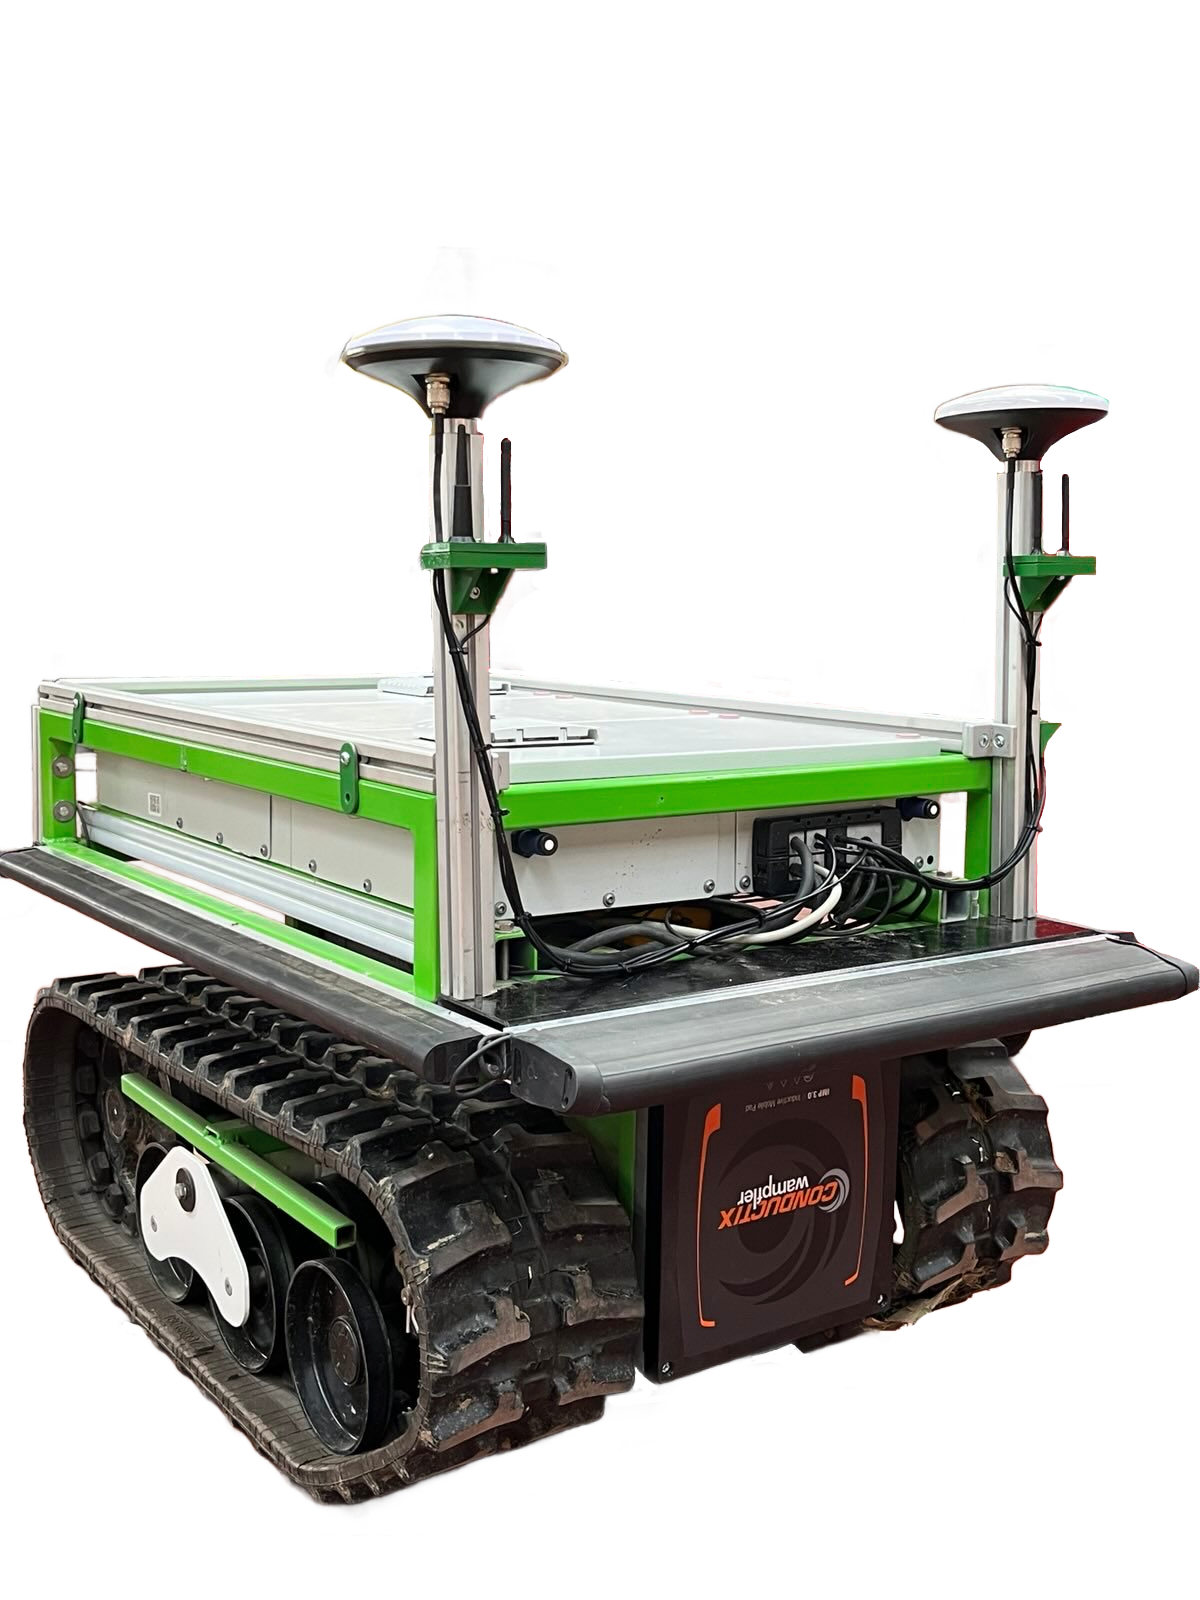
\includegraphics[width=0.5\textwidth]{treebot.png}
    \caption[Treebot ILVO.]{\label{fig:treebot}Treebot ILVO.}
\end{figure}

De robot beschikt over een arm en sensoren om druiven te inspecteren. Om een taak autonoom uit te voeren zijn momenteel drie controlesystemen nodig: navigatiecontrole, actuatorcontrole en taakcontrole. Het RL-algoritme moet deze controllers samenvoegen tot één geïntegreerde controller zodat de robot zelfstandig beslissingen kan nemen, afhankelijk van de situatie.

Om correcte beslissingen te nemen, heeft het RL-algoritme duidelijke omgevingsinformatie nodig. Dit betekent dat de robot druivenranken en -trossen rondom zich moet herkennen. Op Treebot wordt hiervoor een cameraplatform gemonteerd. De bachelorproef draagt bij aan de interpretatie van deze beelden en de vegetatie door semantische segmentatie toe te passen.

Het trainen van een dergelijk model is niet vanzelfsprekend, aangezien een grote hoeveelheid gelabelde data nodig is. Dit vormt een uitdaging voor semantische segmentatie in elke sector, maar in een wijngaardcontext is dit nog lastiger. De planten hebben een complexe, organische structuur met overlappende bladeren en variabele vormen, wat het labelen op pixelniveau bijzonder uitdagend maakt. Het correct onderscheiden van druivenranken en -trossen ten opzichte van de achtergrond vraagt daarom meer precisie en inspanning dan bij objecten met duidelijke contouren. Binnen deze bachelorproef wordt onderzocht in welke mate synthetische data kan bijdragen aan het opvangen van dit tekort en het efficiënter maken van het trainingsproces.

\section{\IfLanguageName{dutch}{Probleemstelling}{Problem Statement}}%
\label{sec:probleemstelling}

Treebot, de landbouwrobot van ILVO, heeft visuele waarneming nodig om zelfstandig in wijngaarden te werken. Om een gepaste actie te kiezen, moet de robot kunnen zien waar de druivenranken en -trossen zich bevinden. Machinevisie kan dit mogelijk maken, specifiek in de vorm van semantische segmentatie. Hierdoor kan hij de gewassen herkennen en onderscheiden van de achtergrond.

Het semantische segmentatiemodel moet in realtime de druivenranken en -trossen kunnen segmenteren. De implementatie van dergelijke modellen op edge devices, zoals kleine landbouwrobots, vormt een uitdaging vanwege beperkte rekenkracht en geheugen. Daarnaast presteren deze modellen vaak minder goed in een landbouwcontext, omdat hun architectuur niet is afgestemd op de complexiteit en variabiliteit van natuurlijke omgevingen. Het grootste struikelblok blijft echter het beperkte aantal beschikbare en gelabelde datasets. Het annoteren van wijngaardbeelden is namelijk een zeer tijdrovend en arbeidsintensief proces. Dit bemoeilijkt de training en generalisatie van een model aanzienlijk.

\section{\IfLanguageName{dutch}{Onderzoeksvraag}{Research question}}%
\label{sec:onderzoeksvraag}

Bovenstaande knelpunten leiden tot de hoofdonderzoeksvraag van deze bachelorproef: \emph{'Hoe kan een deep learning-model worden toegepast voor realtime segmentatie van druivenranken en -trossen in wijngaarden, en hoe draagt synthetische data bij aan de generalisatie?'} 

Om bovenstaande onderzoeksvraag te beantwoorden, worden verschillende deelaspecten onderzocht. Deze staan geformuleerd in de volgende deelvragen:

\begin{itemize}
    \setlength{\itemsep}{0pt}
    \setlength{\parskip}{0pt}
    % \item Wat zijn de natuurlijke en visuele kenmerken van een wijngaard?
    \item Welke uitdagingen ondervinden segmentatiemodellen bij toepassing in de landbouw?
    \item Welke modellen zijn geschikt voor druivenranken en -trossen?
    \item Op welke manier dient synthetische data samengesteld te worden om het segmentatiemodel beter te trainen?
    \item Hoe kan modeloptimalisatie plaatsvinden om segmentatie in realtime op edge devices mogelijk te maken?
\end{itemize}

Samen vormen ze de basis voor het verdere verloop van dit werk.

\section{\IfLanguageName{dutch}{Onderzoeksdoelstelling}{Research objective}}%
\label{sec:onderzoeksdoelstelling}

Het eindresultaat is een proof-of-concept van het segmentatiemodel, gericht op het herkennen van gewassen in wijngaarden. Daarbij is rekening gehouden met de hardwarebeperkingen van de landbouwrobot. De visuele invoer waarop het model werd getraind, bestaat grotendeels uit synthetische beelden. De modelprestaties en evaluatieresultaten in dit onderzoek bepalen in welke mate synthetische data bijdraagt aan een verbeterde generalisatie van het model. Zo wordt duidelijk of synthetische data bruikbaar is bij een tekort aan gelabelde wijngaarddata.

\section{\IfLanguageName{dutch}{Opzet van deze bachelorproef}{Structure of this bachelor thesis}}%
\label{sec:opzet-bachelorproef}

De bachelorproef is als volgt opgebouwd:

In Hoofdstuk~\ref{ch:stand-van-zaken} wordt een overzicht gegeven van de stand van zaken binnen het onderzoeksdomein, op basis van een literatuurstudie.

In Hoofdstuk~\ref{ch:methodologie} worden de methodologie en onderzoekstechnieken besproken, samen met een antwoord op de eerste twee deelvragen.

% TODO: Vul hier aan voor je eigen hoofstukken, één of twee zinnen per hoofdstuk

In Hoofdstuk~\ref{ch:synthetische-data} wordt de synthetische data verzameld door gesimuleerde afbeeldingen te genereren. De labels worden hierbij automatisch bekomen.

In Hoofdstuk~\ref{ch:proof-of-concept} wordt het semantische segmentatiemodel uitgewerkt. Eerst volgt een evaluatie na training met reële data, daarna een tweede evaluatie met toevoeging van synthetische data.

In Hoofdstuk~\ref{ch:conclusie}, tenslotte, wordt de conclusie gegeven en een antwoord geformuleerd op de onderzoeksvragen. Daarbij wordt ook een aanzet gegeven voor toekomstig onderzoek binnen dit domein.
\chapter{\IfLanguageName{dutch}{Stand van zaken}{State of the art}}%
\label{ch:stand-van-zaken}

% Tip: Begin elk hoofdstuk met een paragraaf inleiding die beschrijft hoe
% dit hoofdstuk past binnen het geheel van de bachelorproef. Geef in het
% bijzonder aan wat de link is met het vorige en volgende hoofdstuk.

% Pas na deze inleidende paragraaf komt de eerste sectiehoofding.

Dit hoofdstuk bevat je literatuurstudie. De inhoud gaat verder op de inleiding, maar zal het onderwerp van de bachelorproef *diepgaand* uitspitten. De bedoeling is dat de lezer na lezing van dit hoofdstuk helemaal op de hoogte is van de huidige stand van zaken (state-of-the-art) in het onderzoeksdomein. Iemand die niet vertrouwd is met het onderwerp, weet nu voldoende om de rest van het verhaal te kunnen volgen, zonder dat die er nog andere informatie moet over opzoeken \autocite{Pollefliet2011}.

Je verwijst bij elke bewering die je doet, vakterm die je introduceert, enz.\ naar je bronnen. In \LaTeX{} kan dat met het commando \texttt{$\backslash${textcite\{\}}} of \texttt{$\backslash${autocite\{\}}}. Als argument van het commando geef je de ``sleutel'' van een ``record'' in een bibliografische databank in het Bib\LaTeX{}-formaat (een tekstbestand). Als je expliciet naar de auteur verwijst in de zin (narratieve referentie), gebruik je \texttt{$\backslash${}textcite\{\}}. Soms is de auteursnaam niet expliciet een onderdeel van de zin, dan gebruik je \texttt{$\backslash${}autocite\{\}} (referentie tussen haakjes). Dit gebruik je bv.~bij een citaat, of om in het bijschrift van een overgenomen afbeelding, broncode, tabel, enz. te verwijzen naar de bron. In de volgende paragraaf een voorbeeld van elk.

\textcite{Knuth1998} schreef een van de standaardwerken over sorteer- en zoekalgoritmen. Experten zijn het erover eens dat cloud computing een interessante opportuniteit vormen, zowel voor gebruikers als voor dienstverleners op vlak van informatietechnologie~\autocite{Creeger2009}.

Let er ook op: het \texttt{cite}-commando voor de punt, dus binnen de zin. Je verwijst meteen naar een bron in de eerste zin die erop gebaseerd is, dus niet pas op het einde van een paragraaf.

\begin{figure}
  \centering
  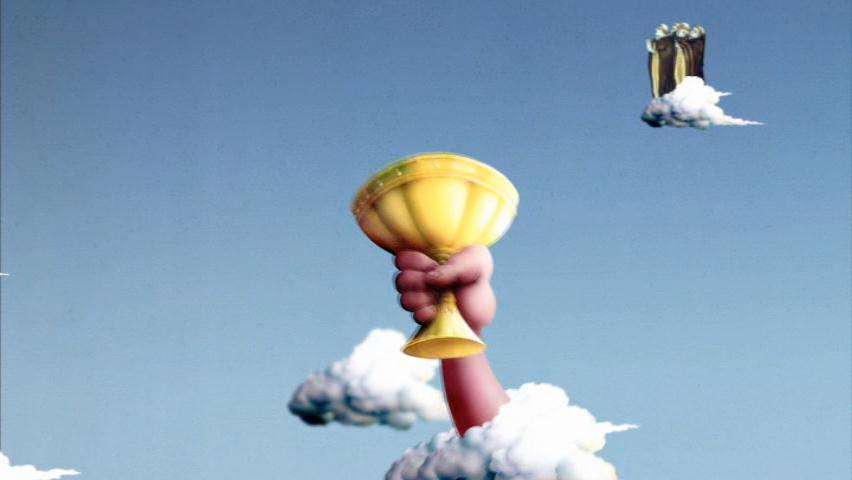
\includegraphics[width=0.8\textwidth]{grail.jpg}
  \caption[Voorbeeld figuur.]{\label{fig:grail}Voorbeeld van invoegen van een figuur. Zorg altijd voor een uitgebreid bijschrift dat de figuur volledig beschrijft zonder in de tekst te moeten gaan zoeken. Vergeet ook je bronvermelding niet!}
\end{figure}

\begin{listing}
  \begin{minted}{python}
    import pandas as pd
    import seaborn as sns

    penguins = sns.load_dataset('penguins')
    sns.relplot(data=penguins, x="flipper_length_mm", y="bill_length_mm", hue="species")
  \end{minted}
  \caption[Voorbeeld codefragment]{Voorbeeld van het invoegen van een codefragment.}
\end{listing}

\lipsum[7-20]

\begin{table}
  \centering
  \begin{tabular}{lcr}
    \toprule
    \textbf{Kolom 1} & \textbf{Kolom 2} & \textbf{Kolom 3} \\
    $\alpha$         & $\beta$          & $\gamma$         \\
    \midrule
    A                & 10.230           & a                \\
    B                & 45.678           & b                \\
    C                & 99.987           & c                \\
    \bottomrule
  \end{tabular}
  \caption[Voorbeeld tabel]{\label{tab:example}Voorbeeld van een tabel.}
\end{table}


%%=============================================================================
%% Methodologie
%%=============================================================================

\chapter{\IfLanguageName{dutch}{Methodologie}{Methodology}}%
\label{ch:methodologie}

%% TODO: In dit hoofstuk geef je een korte toelichting over hoe je te werk bent
%% gegaan. Verdeel je onderzoek in grote fasen, en licht in elke fase toe wat
%% de doelstelling was, welke deliverables daar uit gekomen zijn, en welke
%% onderzoeksmethoden je daarbij toegepast hebt. Verantwoord waarom je
%% op deze manier te werk gegaan bent.
%% 
%% Voorbeelden van zulke fasen zijn: literatuurstudie, opstellen van een
%% requirements-analyse, opstellen long-list (bij vergelijkende studie),
%% selectie van geschikte tools (bij vergelijkende studie, "short-list"),
%% opzetten testopstelling/PoC, uitvoeren testen en verzamelen
%% van resultaten, analyse van resultaten, ...
%%
%% !!!!! LET OP !!!!!
%%
%% Het is uitdrukkelijk NIET de bedoeling dat je het grootste deel van de corpus
%% van je bachelorproef in dit hoofstuk verwerkt! Dit hoofdstuk is eerder een
%% kort overzicht van je plan van aanpak.
%%
%% Maak voor elke fase (behalve het literatuuronderzoek) een NIEUW HOOFDSTUK aan
%% en geef het een gepaste titel.

\begin{listing}
    \begin{minted}{python}
        import pandas as pd
        import seaborn as sns
        
        penguins = sns.load_dataset('penguins')
        sns.relplot(data=penguins, x="flipper_length_mm", y="bill_length_mm", hue="species")
    \end{minted}
    \caption[Voorbeeld codefragment]{Voorbeeld van het invoegen van een codefragment.}
\end{listing}

\begin{table}
    \centering
    \begin{tabular}{lcr}
        \toprule
        \textbf{Kolom 1} & \textbf{Kolom 2} & \textbf{Kolom 3} \\
        $\alpha$         & $\beta$          & $\gamma$         \\
        \midrule
        A                & 10.230           & a                \\
        B                & 45.678           & b                \\
        C                & 99.987           & c                \\
        \bottomrule
    \end{tabular}
    \caption[Voorbeeld tabel]{\label{tab:example}Voorbeeld van een tabel.}
\end{table}

\lipsum[21-25]


% Voeg hier je eigen hoofdstukken toe die de ``corpus'' van je bachelorproef
% vormen. De structuur en titels hangen af van je eigen onderzoek. Je kan bv.
% elke fase in je onderzoek in een apart hoofdstuk bespreken.

%\input{...}
%\input{...}
%...

%%=============================================================================
%% Conclusie
%%=============================================================================

\chapter{Conclusie}%
\label{ch:conclusie}

% TODO: Trek een duidelijke conclusie, in de vorm van een antwoord op de
% onderzoeksvra(a)g(en). Wat was jouw bijdrage aan het onderzoeksdomein en
% hoe biedt dit meerwaarde aan het vakgebied/doelgroep? 
% Reflecteer kritisch over het resultaat. In Engelse teksten wordt deze sectie
% ``Discussion'' genoemd. Had je deze uitkomst verwacht? Zijn er zaken die nog
% niet duidelijk zijn?
% Heeft het onderzoek geleid tot nieuwe vragen die uitnodigen tot verder 
%onderzoek?

\lipsum[76-80]



%---------- Bijlagen -----------------------------------------------------------

\appendix

\chapter{Onderzoeksvoorstel}

Het onderwerp van deze bachelorproef is gebaseerd op een onderzoeksvoorstel dat vooraf werd beoordeeld door de promotor. Dat voorstel is opgenomen in deze bijlage.

%% TODO: 
\section*{Samenvatting}

% Kopieer en plak hier de samenvatting (abstract) van je onderzoeksvoorstel.
AI biedt het potentieel om autonome landbouwtechnologieën verder te moderniseren. De landbouwsector blijkt echter moeilijk toegankelijk voor de implementatie van bestaande AI-oplossingen. Dit komt vooral door de complexiteit en variabiliteit van natuurlijke omgevingen. Een specifieke uitdaging binnen dit domein is de realtime segmentatie van druivenplanten, mede door het tekort aan (gelabelde) datasets. Dit leidt tot de hoofdonderzoeksvraag: \emph{'Hoe kan een deep learning model worden toegepast voor realtime segmentatie van druivenranken en -trossen in wijngaarden, en hoe draagt gesynthetiseerde data bij aan de generalisatie?'} Deze bachelorproef richt zich op de ontwikkeling en training van een segmentatiemodel met data afkomstig uit zowel echte als gesimuleerde wijngaarden. Het model wordt iteratief bijgesteld op basis van evaluaties om de prestaties te optimaliseren. Het einddoel is een model dat geschikt is voor realtime toepassingen. Deze aanpak zal naar verwachting leiden tot een praktisch toepasbaar segmentatiemodel.  Het gebruik van gesynthetiseerde data zal naar veronderstelling de generalisatie van het model positief beïnvloeden. Bovendien bewijst gesynthetiseerde data zijn waarde als aanvullende bron wanneer echte landbouwdata moeilijk beschikbaar is.

% Verwijzing naar het bestand met de inhoud van het onderzoeksvoorstel
%---------- Inleiding ---------------------------------------------------------

% TODO: Is dit voorstel gebaseerd op een paper van Research Methods die je
% vorig jaar hebt ingediend? Heb je daarbij eventueel samengewerkt met een
% andere student?
% Zo ja, haal dan de tekst hieronder uit commentaar en pas aan.

%\paragraph{Opmerking}

% Dit voorstel is gebaseerd op het onderzoeksvoorstel dat werd geschreven in het
% kader van het vak Research Methods dat ik (vorig/dit) academiejaar heb
% uitgewerkt (met medesturent VOORNAAM NAAM als mede-auteur).
% 

\section{Inleiding}%
\label{sec:inleiding}

Twintig jaar geleden was er nauwelijks sprake van Belgische wijnbouw. De laatste jaren is deze sector echter uitgegroeid tot een productieve pijler binnen onze landbouw. Volgens \textcite{FODEconomie2024} werd er in 2023 meer dan 3,4 miljoen liter wijn geproduceerd, en de productie blijft groeien. Het aantal hectaren neemt ook elk jaar toe. Daarom krijgt deze sector aandacht binnen het\textit{ Flanders AI Research Programme} (FAIR). FAIR is een consortium van onderzoeksgroepen aan Vlaamse universiteiten en onderzoekscentra, gericht op AI-onderzoek in diverse Vlaamse sectoren. Het Instituut voor Landbouw-, Visserij- en Voedingsonderzoek (ILVO) is een van deze centra. Samen met UAntwerpen werken zij aan een project om de druivenkwaliteit in wijngaarden autonoom te monitoren met behulp van AI.

Voor dit project wordt een reinforcement learning (RL)-algoritme ontwikkeld, dat op een kleine landbouwrobot wordt geïmplementeerd. De robot is uitgerust met een arm en sensoren om druiven te meten. Hij kan reeds autonoom monitoren op basis van drie controllers: navigatie, besturing en taakuitvoering. Het RL-model moet deze controllers combineren tot één geïntegreerde controller, waardoor de robot zelfstandig beslissingen kan maken, afhankelijk van de situatie.

Een belangrijk knelpunt in dit project is het ontbreken van een omgevingskaart. Het RL-model heeft deze kaart nodig om zijn toestand te kunnen waarnemen en zo de beste acties te bepalen. Een gesegmenteerde 2D-kaart kan hiervoor een oplossing bieden. Een mogelijke aanpak is om gekalibreerde puntenwolken in te kleuren met informatie uit gesegmenteerde beelden en deze punten vervolgens in 2D te projecteren. Deze bachelorproef draagt bij aan de ontwikkeling van deze kaart door de semantische segmentatie van beelden uit wijngaarden te realiseren.

Het semantische segmentatiemodel moet op de robot kunnen draaien en gewassen nauwkeurig segmenteren, wat niet vanzelfsprekend is. Dergelijke modellen vereisen veel rekenkracht en geheugen. Bovendien presteren ze vaak minder goed in landbouwomgevingen vanwege de modelarchitecturen, unieke kenmerken van landbouwafbeeldingen en het gebrek aan (gelabelde) landbouwdatasets. Dit leidt tot de hoofdonderzoeksvraag: \emph{'Hoe kan een deep learning model worden toegepast voor nauwkeurige en efficiënte segmentatie van gewassen in een wijngaard, en hoe draagt gesimuleerde data bij aan de generalisatie?'}

Binnen het probleemgebied wordt onderzocht welke unieke kenmerken wijngaardafbeeldingen hebben en welke uitdagingen deze vormen voor de segmentatie. Daarnaast wordt gekeken naar welk model geschikt is voor segmentatie binnen de context van wijngaarden.

In het oplossingsgebied ligt de focus op praktische modelverbetering. Er wordt onderzocht hoe virtueel gegenereerde data de beperkte echte data kan aanvullen en hoe (semi-)automatische datalabeling kan worden toegepast op beide soorten data. Daarnaast wordt gekeken naar de modeloptimalisatie voor toepassing op de robot.

Het eindresultaat van de bachelorproef is een proof-of-concept van het afgestemde segmentatiemodel voor de robot, dat gewassen in de wijngaard kan segmenteren. Het model zal worden beoordeeld op efficiëntie en nauwkeurigheid.

%---------- Stand van zaken ---------------------------------------------------

\section{Literatuurstudie}%
\label{sec:literatuurstudie}

Hier beschrijf je de \emph{state-of-the-art} rondom je gekozen onderzoeksdomein, d.w.z.\ een inleidende, doorlopende tekst over het onderzoeksdomein van je bachelorproef. Je steunt daarbij heel sterk op de professionele \emph{vakliteratuur}, en niet zozeer op populariserende teksten voor een breed publiek. Wat is de huidige stand van zaken in dit domein, en wat zijn nog eventuele open vragen (die misschien de aanleiding waren tot je onderzoeksvraag!)?

Je mag de titel van deze sectie ook aanpassen (literatuurstudie, stand van zaken, enz.). Zijn er al gelijkaardige onderzoeken gevoerd? Wat concluderen ze? Wat is het verschil met jouw onderzoek?

Verwijs bij elke introductie van een term of bewering over het domein naar de vakliteratuur, bijvoorbeeld~\autocite{Hykes2013}! Denk zeker goed na welke werken je refereert en waarom.

Draag zorg voor correcte literatuurverwijzingen! Een bronvermelding hoort thuis \emph{binnen} de zin waar je je op die bron baseert, dus niet er buiten! Maak meteen een verwijzing als je gebruik maakt van een bron. Doe dit dus \emph{niet} aan het einde van een lange paragraaf. Baseer nooit teveel aansluitende tekst op eenzelfde bron.

Als je informatie over bronnen verzamelt in JabRef, zorg er dan voor dat alle nodige info aanwezig is om de bron terug te vinden (zoals uitvoerig besproken in de lessen Research Methods).

% Voor literatuurverwijzingen zijn er twee belangrijke commando's:
% \autocite{KEY} => (Auteur, jaartal) Gebruik dit als de naam van de auteur
%   geen onderdeel is van de zin.
% \textcite{KEY} => Auteur (jaartal)  Gebruik dit als de auteursnaam wel een
%   functie heeft in de zin (bv. ``Uit onderzoek door Doll & Hill (1954) bleek
%   ...'')

Je mag deze sectie nog verder onderverdelen in subsecties als dit de structuur van de tekst kan verduidelijken.

%---------- Methodologie ------------------------------------------------------
\section{Methodologie}%
\label{sec:methodologie}

Tijdens de \textbf{eerste fase} ligt de focus op het verzamelen, analyseren, simuleren en labelen van data. Echte data wordt verzameld via camera of uit bestaande datasets, terwijl virtuele wijngaarden worden ontworpen in Blender. De visuele kenmerken van wijngaardbeelden komen naar voren. Het labelen van de gewassen zal (gedeeltelijk) automatisch verlopen via Roboflow. Dit leidt tot een gecombineerde dataset van reële en gesynthetiseerde data, specifiek gericht op de segmentatie van druivenplanten. Deze fase is acht weken lang.

De \textbf{tweede fase} richt zich op de ontwikkeling van het model en de impact van gesimuleerde data. Na een literatuuronderzoek naar segmentatie-uitdagingen in wijngaard- en landbouwdata volgt de selectie van een geschikt semantisch segmentatiemodel. Dit model wordt geïmplementeerd met behulp van Keras of GitHub-repositories. Training gebeurt eerst uitsluitend met echte data en wordt vervolgens aangevuld met gesimuleerde data. Naast de algemene modelbeoordeling vindt een evaluatie plaats om te bepalen of virtuele data de generalisatie van het model versterkt. Deze fase resulteert in een afgestemd segmentatiemodel voor gewassen in wijngaarden en neemt vier weken in beslag.

De \textbf{derde en laatste fase} concentreert zich op de optimalisatie van het model voor veldtoepassingen. Met technieken zoals pruning en quantization wordt het model geschikt gemaakt voor gebruik op een robot met beperkte rekenkracht. Een eindbeoordeling van het geoptimaliseerde model sluit het proces af. Deze slotfase duurt twee weken.

%---------- Verwachte resultaten ----------------------------------------------
\section{Verwacht resultaat, conclusie}%
\label{sec:verwachte_resultaten}

Hier beschrijf je welke resultaten je verwacht. Als je metingen en simulaties uitvoert, kan je hier al mock-ups maken van de grafieken samen met de verwachte conclusies. Benoem zeker al je assen en de onderdelen van de grafiek die je gaat gebruiken. Dit zorgt ervoor dat je concreet weet welk soort data je moet verzamelen en hoe je die moet meten.

Wat heeft de doelgroep van je onderzoek aan het resultaat? Op welke manier zorgt jouw bachelorproef voor een meerwaarde?

Hier beschrijf je wat je verwacht uit je onderzoek, met de motivatie waarom. Het is \textbf{niet} erg indien uit je onderzoek andere resultaten en conclusies vloeien dan dat je hier beschrijft: het is dan juist interessant om te onderzoeken waarom jouw hypothesen niet overeenkomen met de resultaten.



%%---------- Andere bijlagen --------------------------------------------------
% TODO: Voeg hier eventuele andere bijlagen toe. Bv. als je deze BP voor de
% tweede keer indient, een overzicht van de verbeteringen t.o.v. het origineel.
%\input{...}

%%---------- Backmatter, referentielijst ---------------------------------------

\backmatter{}

\setlength\bibitemsep{2pt} %% Add Some space between the bibliograpy entries
\printbibliography[heading=bibintoc]

\end{document}
